\input{../../odp_latex_codes/begindoc.tex}

\section*{Example: ``ex001''}



\textbf{Remark:} Example of the paper optdes.

\input{../../odp_latex_codes/nscd.tex}

\begin{sloppypar}

${A=\dots}$, 
${k=4}$, 
${\tau=0.8}$, 
${\mu=0.9}$, 
${\gamma1=1}$, 
${\gamma2=3}$, 
${b=\begin{pmatrix}
50\\
40
\end{pmatrix}
}$, 
${c=\begin{pmatrix}
1\\
1\\
1\\
1\\
2\\
2\\
3\\
3\\
2\\
2\\
2\\
2\\
3\\
3\\
2\\
2\\
6\\
6
\end{pmatrix}
}$, 
${u=\begin{pmatrix}
24\\
24\\
12\\
12\\
13\\
13\\
18\\
18\\
15\\
15\\
26\\
26\\
17\\
17\\
23\\
23\\
8\\
8
\end{pmatrix}
}$, 
${a=\begin{pmatrix}
10\\
11\\
8\\
9
\end{pmatrix}
}$, 
\end{sloppypar}

\newpage

\subsection*{Design process}

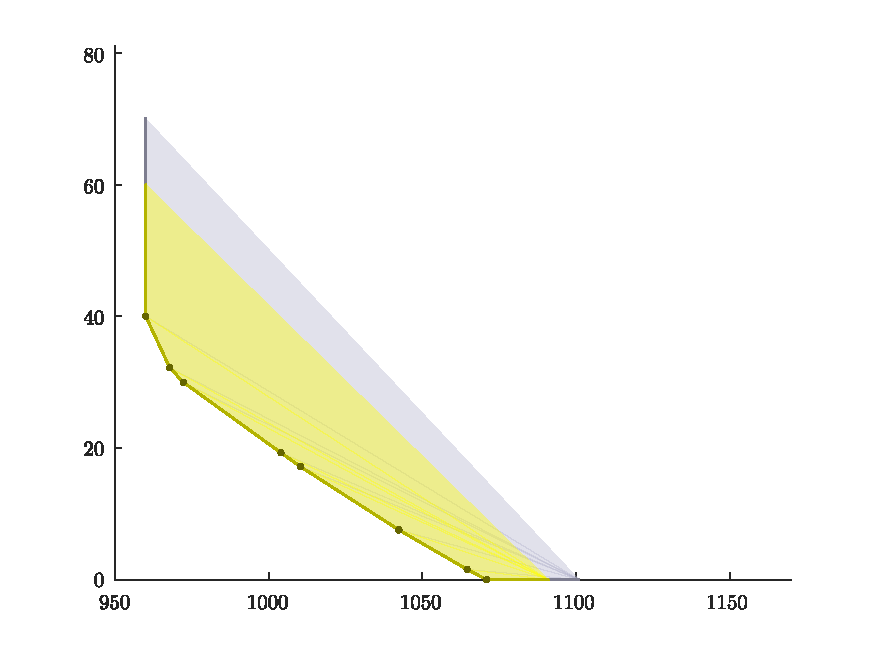
\includegraphics[width=0.5\textwidth]{plot1.pdf} 
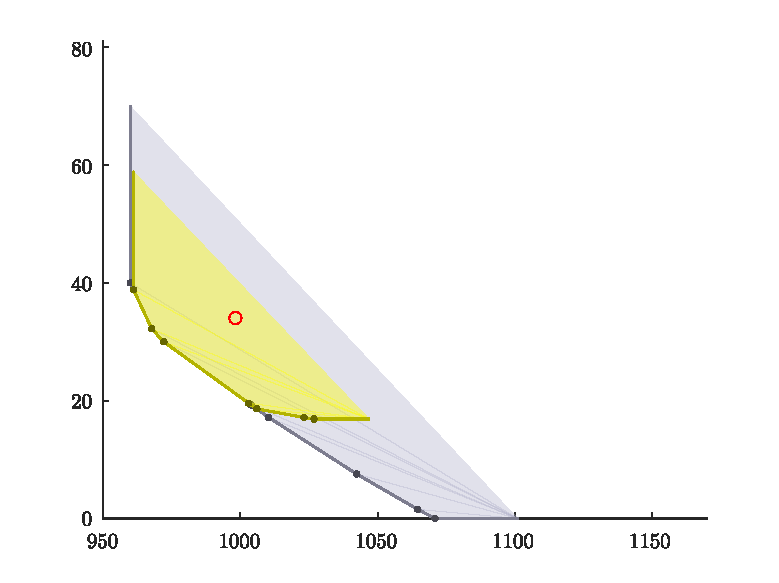
\includegraphics[width=0.5\textwidth]{plot2.pdf} 
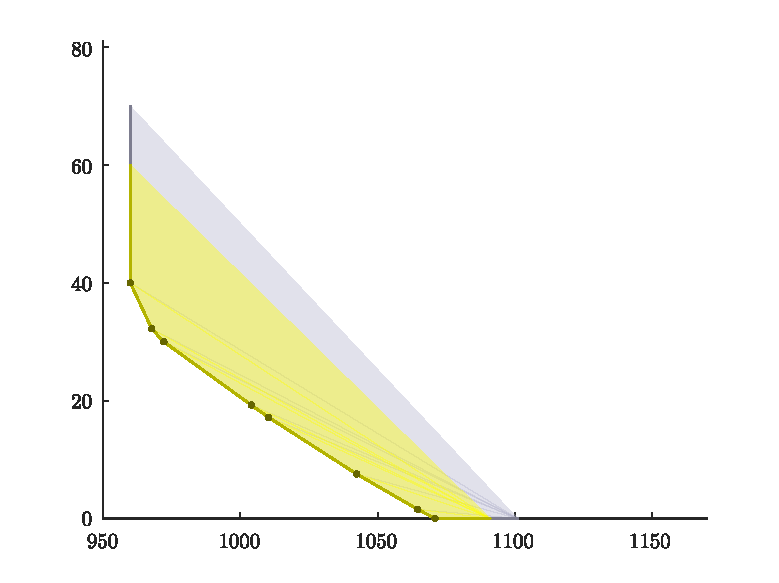
\includegraphics[width=0.5\textwidth]{plot3.pdf} 
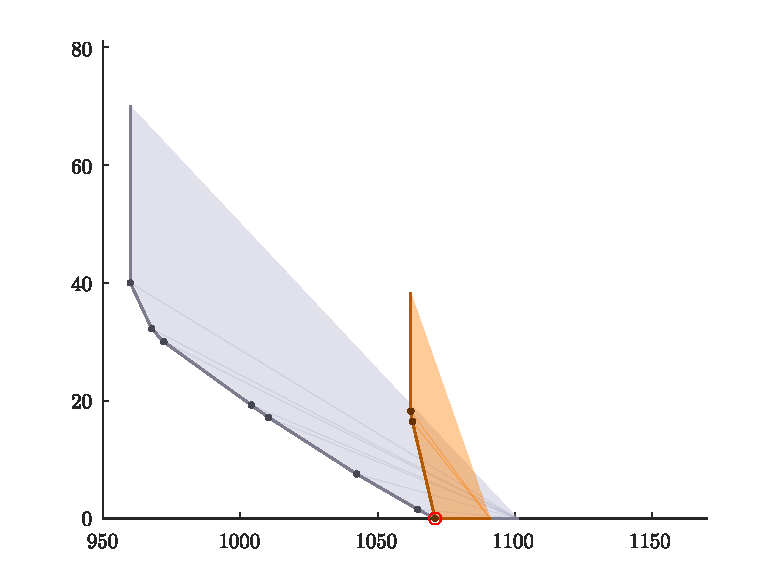
\includegraphics[width=0.5\textwidth]{plot4.pdf} 
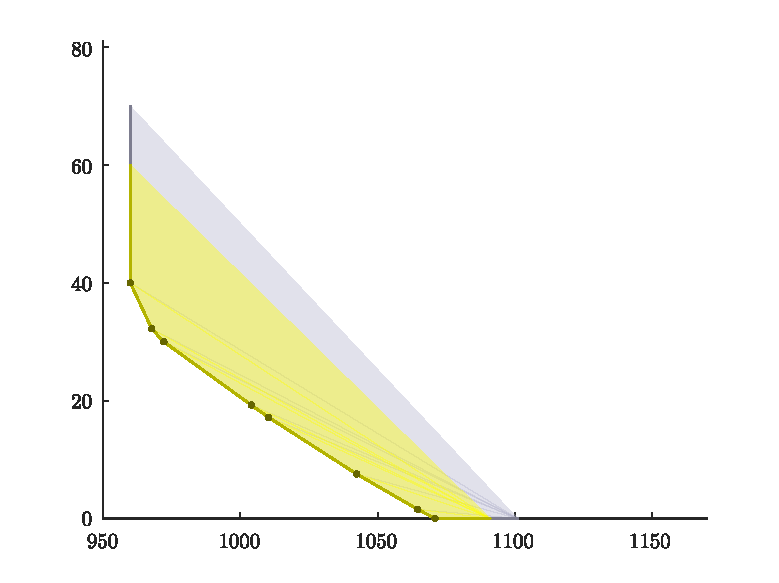
\includegraphics[width=0.5\textwidth]{plot5.pdf} 
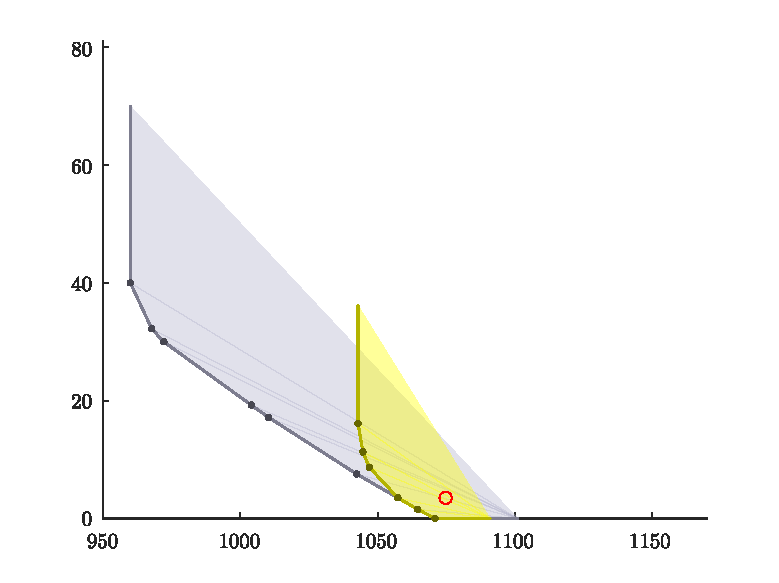
\includegraphics[width=0.5\textwidth]{plot6.pdf} 
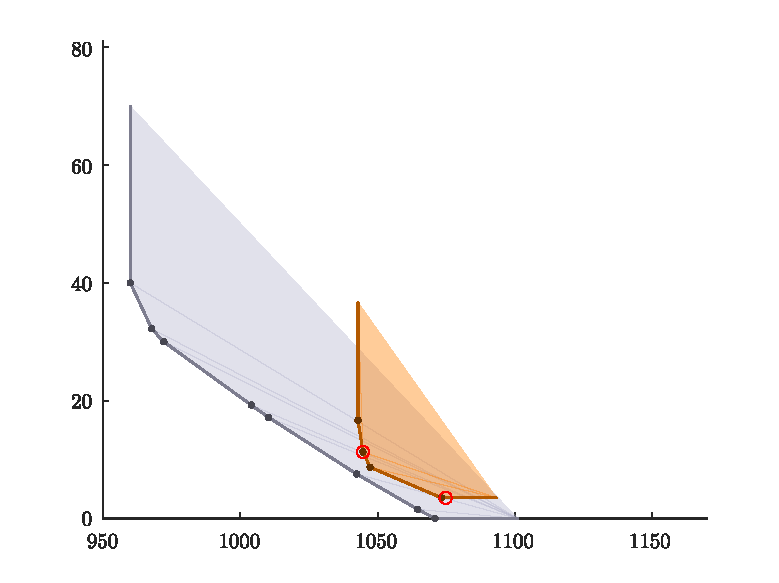
\includegraphics[width=0.5\textwidth]{plot7.pdf} 
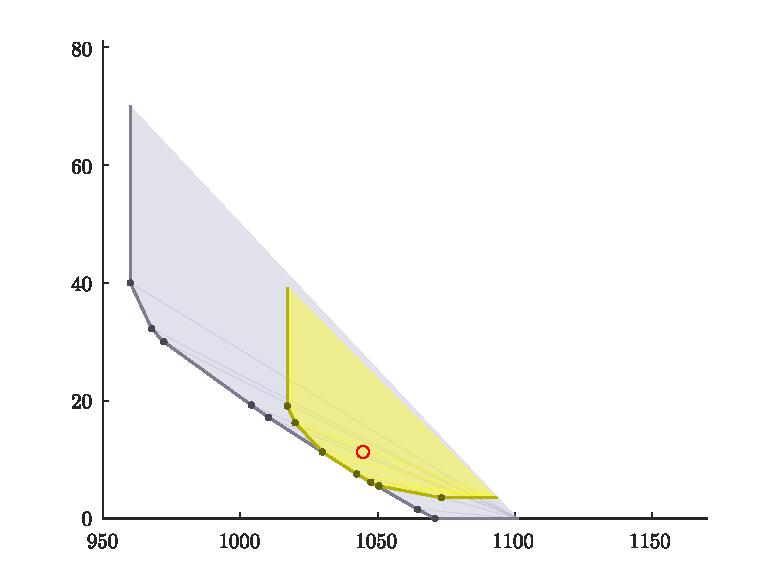
\includegraphics[width=0.5\textwidth]{plot8.pdf} 
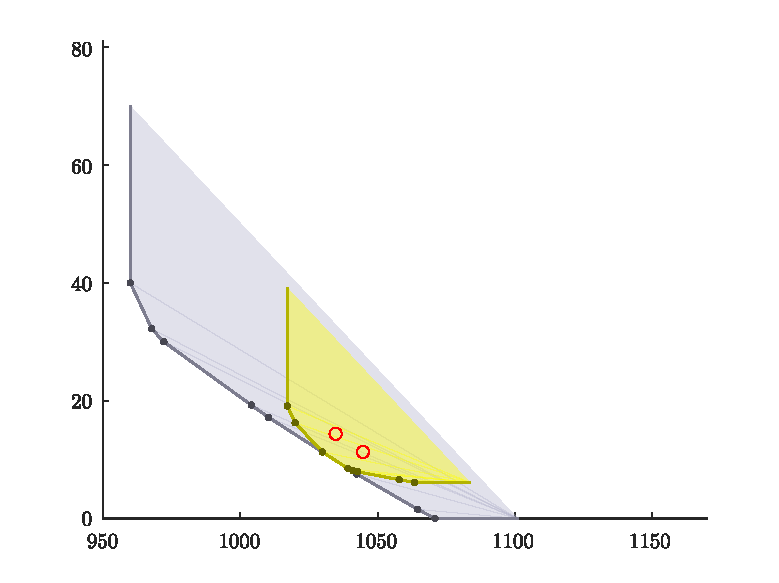
\includegraphics[width=0.5\textwidth]{plot9.pdf} 
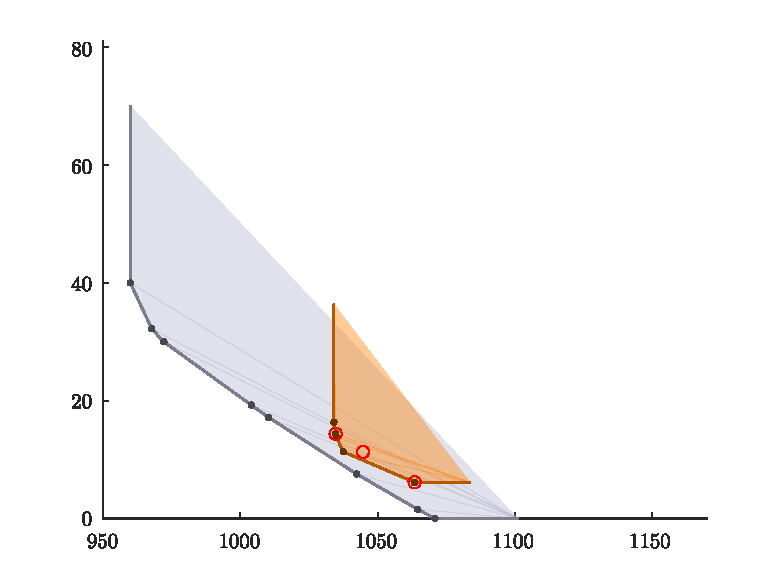
\includegraphics[width=0.5\textwidth]{plot10.pdf} 
\begin{sloppypar}

${z=\begin{pmatrix}
22.2222222224635&29.5917810887544&28.4491187066995\\
5.77777777774142&0&0\\
36.4444444444444&36.4444444444444&36.4444444444444\\
35.5555555553143&32.6666666666249&32.8343353051141
\end{pmatrix}
}$, 
\end{sloppypar}

\begin{sloppypar}

${Y_1=\begin{pmatrix}

\end{pmatrix}
}$, 
${Y_2=\begin{pmatrix}
998.258064516129\\
34.0280455740578
\end{pmatrix}
}$, 
${Y_3=\begin{pmatrix}

\end{pmatrix}
}$, 
${Y_4=\begin{pmatrix}
1070.93333333297\\
7.90549847806687e-11
\end{pmatrix}
}$, 
${Y_5=\begin{pmatrix}

\end{pmatrix}
}$, 
${Y_6=\begin{pmatrix}
1074.80184331797\\
3.50219106047327
\end{pmatrix}
}$, 
${Y_7=\begin{pmatrix}
1074.80184331797&1044.67336644269\\
3.50219106047327&11.3021910604733
\end{pmatrix}
}$, 
${Y_8=\begin{pmatrix}
1044.67336644269\\
11.3021910604733
\end{pmatrix}
}$, 
${Y_9=\begin{pmatrix}
1044.67336644269&1034.75576036866\\
11.3021910604733&14.387379491674
\end{pmatrix}
}$, 
${Y_10=\begin{pmatrix}
1044.67336644269&1034.75576036866&1063.50666214319\\
11.3021910604733&14.387379491674&6.13467416810513
\end{pmatrix}
}$, 
\end{sloppypar}

\input{../../odp_latex_codes/enddoc.tex}

